\subsection{Outlines reduce secret-word discrimination}
Table~\ref{tab:behavior} and Figure~\ref{fig:behavior} summarize all behavioral pairs. For the primary reader, word-secret discrimination is 81.2\% under plain prompting, 79.6\% with filler, 54.6\% with an outline, and 72.1\% with a decoy. The outline reduces discrimination by 26.7 points relative to plain prompting and 25.0 points relative to filler. Both contrasts survive the planned correction, and item-cluster intervals remain well below zero (Table~\ref{tab:contrasts}). Thus, simply appending a similar amount of irrelevant prose does not reproduce the outline effect.

The secondary reader yields the same ordering among plain, filler, and outline conditions. It refuses some word-secret comparisons, so its main estimates are complete-pair results rather than a fully observed replication. An adversarial assignment of all missing order judgments still separates outline accuracy (49.2--55.4\%) from plain accuracy (81.2--90.8\%). These are missing-data bounds, not confidence intervals. They show that those refusals cannot by themselves reverse the large word-secret difference.

\begin{table*}[t]
\centering\small
\begin{tabular}{llrrr}
\toprule Domain & Condition & Pairs & Sonnet (95\% CI) & Mini (pairs) \\
\midrule
Word & Plain & 120 & 81.2 [76.7, 85.8] & 90.1 (101) \\
Word & Filler & 120 & 79.6 [74.2, 84.6] & 86.5 (100) \\
Word & Outline & 120 & 54.6 [50.8, 58.3] & 52.8 (107) \\
Word & Decoy & 120 & 72.1 [67.1, 77.1] & 82.3 (99) \\
Plot & Plain & 60 & 55.8 [50.0, 61.7] & 57.5 (60) \\
Plot & Filler & 60 & 57.5 [52.5, 62.5] & 65.0 (60) \\
Plot & Outline & 60 & 48.3 [44.2, 52.5] & 51.7 (60) \\
Plot & No Secret & 60 & 46.7 [43.3, 49.2] & 49.2 (60) \\
\bottomrule
\end{tabular}
\caption{Behavioral discrimination in percent. ``Pairs'' counts complete primary-reader pairs. Mini reports complete-pair accuracy with its own pair count in parentheses. Intervals bootstrap pairs, retaining both orders together. The plot no-secret primary-reader interval has a boundary artifact discussed in the text.}
\label{tab:behavior}
\end{table*}
\begin{figure*}[t]
\centering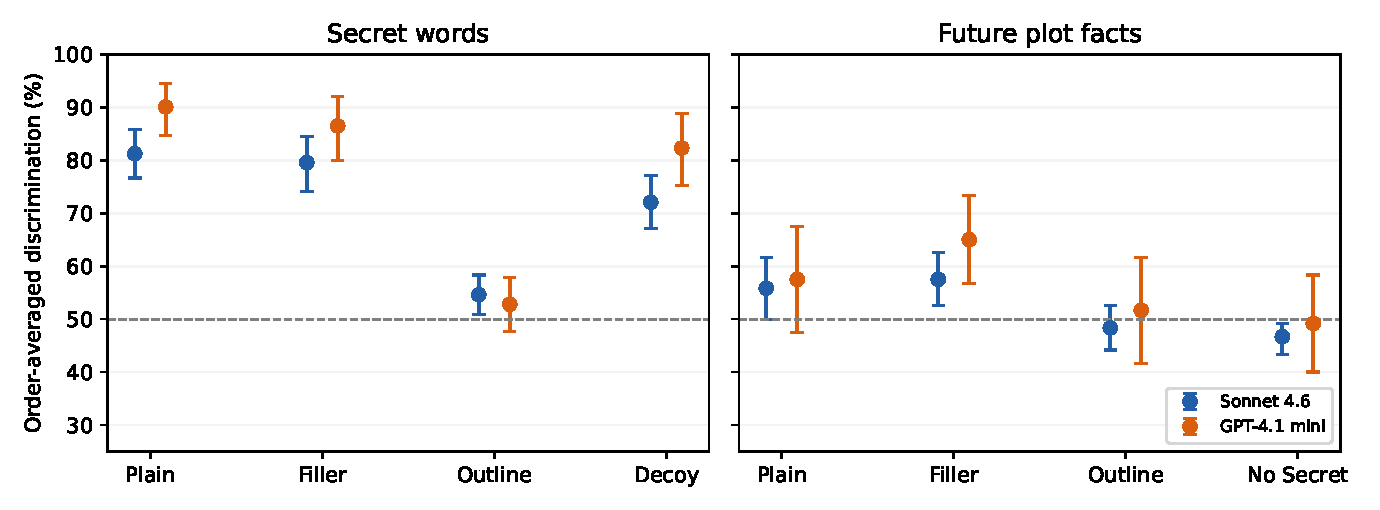
\includegraphics[width=.94\textwidth]{figures/behavior.pdf}
\caption{Order-averaged discrimination and story-pair bootstrap intervals. Dashed lines denote chance. Outlines markedly reduce secret-word discrimination for both readers; plot results are nearer chance and more reader-dependent. Chance-level performance of a particular reader is not proof that the text contains no information.}
\label{fig:behavior}
\end{figure*}
\begin{table*}[t]
\centering\small
\begin{tabular}{llrrr}
\toprule Domain & Contrast & Difference [95\% CI] & Item CI & $p_{\mathrm{Holm}}$ \\
\midrule
Word & outline-plain & -26.7 [-32.1, -21.2] & [-35.0, -17.9] & $<0.0001$ \\
Word & outline-filler & -25.0 [-30.8, -19.2] & [-34.6, -15.0] & $<0.0001$ \\
Plot & outline-plain & -7.5 [-15.0, -0.8] & [-15.0, -0.8] & 0.0627 \\
Plot & outline-filler & -9.2 [-15.0, -4.2] & [-16.7, -2.5] & 0.0073 \\
\bottomrule
\end{tabular}
\caption{Primary paired contrasts in percentage points. Negative values favor outlines. ``Item CI'' resamples target words or premises rather than individual generation blocks. Holm correction covers the four displayed tests.}
\label{tab:contrasts}
\end{table*}

\subsection{Plot effects are smaller and comparator-dependent}
For future facts, primary-reader accuracy is 55.8\% with plain prompting, 57.5\% with filler, and 48.3\% with the generic outline. The outline--filler contrast is $-9.2$ points with corrected $p=0.0073$; the outline--plain contrast is $-7.5$ points with corrected $p=0.0627$. The latter does not meet a conventional 5\% threshold after the planned correction, despite its percentile interval being negative. The intervals are unadjusted, whereas the reported $p$-values are multiplicity-adjusted; the discrete sign-flip test also need not invert the percentile bootstrap.

The no-secret control scores 46.7\% for Sonnet and 49.2\% for Mini. For Sonnet, 56 pairs receive an order-averaged score of one half and four receive zero; none receive one. Consequently, the empirical percentile bootstrap interval excludes one half even though the two-sided sign-flip calibration test gives $p=0.125$. We do not interpret this boundary behavior as evidence of a real anti-secret signal. The plain plot anchor is itself near chance, limiting the room for a detectable reduction. We therefore do not infer a general solution to plot foreshadowing.

\subsection{Text and measurement diagnostics}
None of the 960 behavioral word stories contains its literal secret, and none of the 1,440 behavioral outputs reaches its token cap. The outline word stories average 489.8 words versus 475.9 with filler, so the large effect does not arise from simply producing shorter stories. The outline and filler prompts average 127.1 and 124.8 Gemma tokens for words, and 180.8 and 179.8 for plots, excluding chat-template overhead. Token lengths are close but not exactly matched.

Within-pair content-word Jaccard overlap, an exploratory lexical diagnostic, rises from 0.082 for plain word stories to 0.198 for outline stories. The corresponding plot values are 0.134 and 0.149. This is consistent with concrete outlines fixing more content decisions, although lexical overlap does not measure internal planning. Behavioral quality ratings all reach the coherence and fluency ceiling; nonrepetition averages are slightly lower under outlines. These scores rule out obvious failures detected by this judge, not subtle literary degradation.

Position sensitivity is substantial. For Sonnet, the same underlying passage is selected in both orders for 65.8\% of plain word pairs but only 17.5\% of outline word pairs. In the plot no-secret control, it selects displayed passage B in 96.7\% of calls. Averaging both orders prevents that default from appearing as high accuracy, but low order consistency warns that the reader may be indecisive. There are 86 secondary-reader content-filter responses, all on word comparisons; the primary reader and both readers' plot judgments are complete.

\subsection{Residual evidence and intervention}
The simple centroid readout is weak on raw held-out residuals, ranging from 25.0\% to 35.4\% across the sampled layers and positions (four-way chance: 25\%). Subtracting a matched no-secret state or the mean over secret counterfactuals changes the result substantially (Figure~\ref{fig:readout}). With oracle secret centering, layer-48 accuracy ranges from 66.7\% to 81.2\%. The three-way equal-token-length oracle check reaches 75.0--86.1\% at that layer (chance: 33.3\%), so this contrast signal is not explained solely by telescope's extra token. This establishes context-dependent identity information under a controlled readout, not a clean, universally accessible secret coordinate.

A post hoc supervised linear probe improves raw-state readout, but remains modest and tends to weaken at later positions. At layer 24, four-way accuracy decreases from 54.2\% at token 64 to 29.2\% at token 576; the equal-length three-way values are 61.1\% and 41.7\%. At that layer, algebraic target projection removal does not make the supervised decoder uniformly fall to chance. The operation is therefore not validated as identity erasure, even at the intervention site. Since the operation itself depends on the secret, post-intervention decodability cannot cleanly distinguish surviving from newly introduced information.

\begin{figure*}[t]
\centering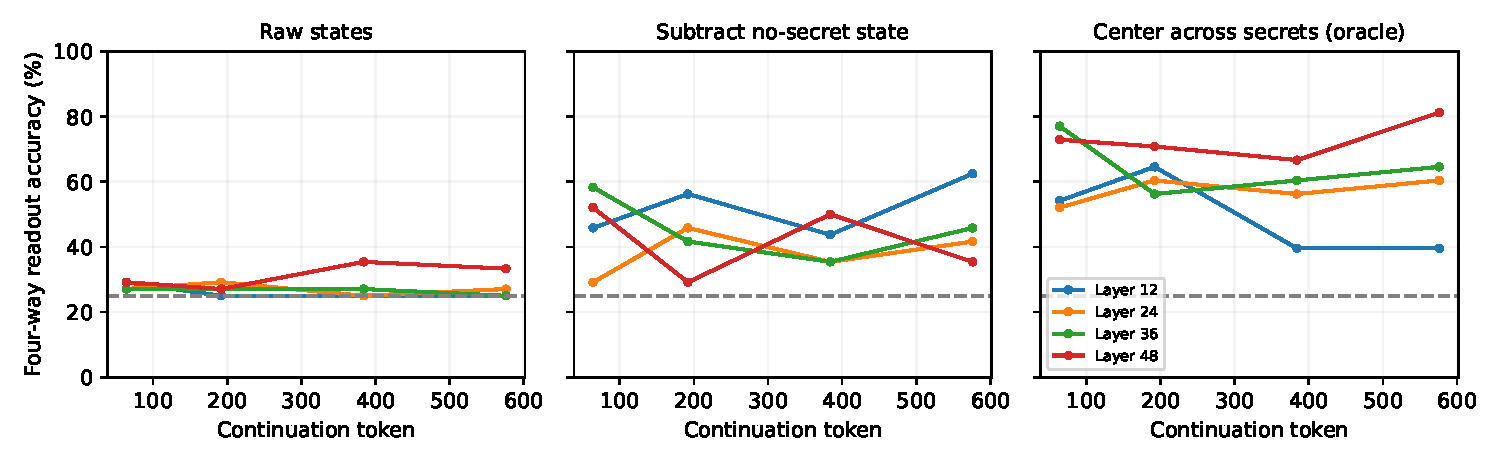
\includegraphics[width=\textwidth]{figures/readout.pdf}
\caption{Secret-identity readout on identical held-out continuations. The large dependence on centering exposes continuation-related nuisance variation. Oracle centering needs all four secret counterfactuals and is not an online decoder. See the appendix for supervised and equal-token-length controls.}
\label{fig:readout}
\end{figure*}

Table~\ref{tab:mechanism} and Figure~\ref{fig:ablation} show the completed local generation experiment. Primary-reader discrimination is 91.7\% at baseline, 95.8\% after target projection removal, 75.0\% under the random control, and 93.8\% under the other-concept control. Target minus baseline is $+4.2$ points (95\% interval: $[-6.2, 16.7]$). The experiment provides no evidence of useful mitigation by the targeted removal. The high local baseline differs from the main study's inventory and generation setup and is not evidence of an API/local implementation effect.

Target removal produces 6 exact-word disclosures among 48 stories, versus 0 at baseline. Removing all baseline--target blocks with a literal disclosure leaves 18 pairs; the exploratory target--baseline contrast is $-2.8$ points (95\% interval: $[-11.1, 5.6]$). This filtered comparison is descriptive because inclusion depends on outcomes. A component involved in secret-dependent behavior need not support concealment when removed.

The random arm's lower discrimination accompanies degraded writing. Mean coherence is 5.00 at baseline, 4.94 for target removal, 3.62 for random removal, and 4.75 for the other-concept arm. Mean fluency is 5.00, 4.69, 3.35, and 4.50, respectively; 8 random-arm outputs reach the token cap. Such a change is not clean evidence of selective leakage removal. Mean perturbation/residual norm ratios during active generation are 2.92\% (target), 5.55\% (random), and 3.17\% (other). The controls match the per-state subtraction rule, but not the realized dose across diverging trajectories.

Baseline pair-averaged activation strength has an exploratory Spearman correlation of $\rho=-0.07$ with primary-reader discrimination ($n=24$, $p=0.733$). This small, high-accuracy sample does not establish a reliable activation--leakage relationship. Taken together, the readouts and interventions show the limits of this particular estimator and ablation, rather than identifying a necessary secret-leakage circuit.

\begin{table*}[t]
\centering\small\begin{tabular}{llrrrrr}
\toprule
Arm & Pairs & Sonnet [95\% CI] & Mini (pairs) & Literal /48 & Coherence & Nonrep. \\
\midrule
Base & 24 & 91.7 [81.2, 100.0] & 87.5 (24) & 0 & 5.00 & 4.27 \\
Target & 24 & 95.8 [89.6, 100.0] & 93.8 (24) & 6 & 4.94 & 4.08 \\
Random & 24 & 75.0 [58.3, 89.6] & 80.4 (23) & 0 & 3.62 & 3.04 \\
Other & 24 & 93.8 [83.3, 100.0] & 95.7 (23) & 0 & 4.75 & 4.02 \\
\bottomrule
\end{tabular}
\caption{Local generation interventions. Discrimination is in percent, with pair-bootstrap intervals. Mini counts include only complete order pairs. Literal disclosures count stories containing the exact secret word; quality means are over all 48 stories per arm.}
\label{tab:mechanism}
\end{table*}
\begin{figure}[t]
\centering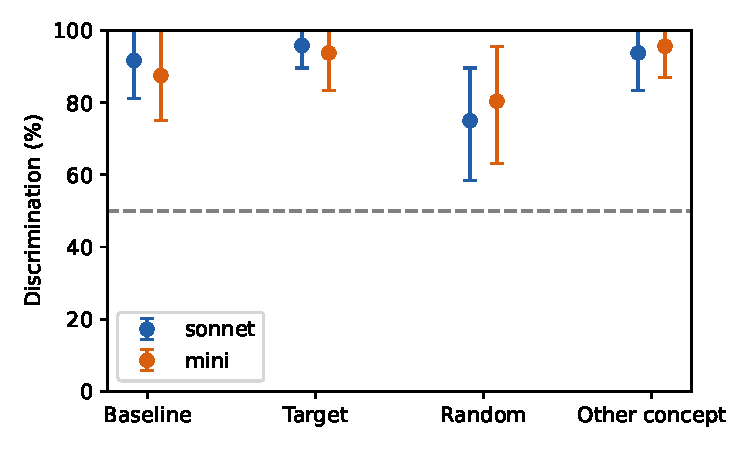
\includegraphics[width=\columnwidth]{figures/ablation.pdf}
\caption{Local intervention discrimination. These arms use four concrete words and 24 pairs each, a smaller and different inventory from the main behavioral study.}
\label{fig:ablation}
\end{figure}

